
\documentclass{llncs}
\usepackage[tbtags]{amsmath}
\usepackage{amsfonts}
\usepackage{algorithm,algorithmic}
\usepackage{mathtools}
\usepackage{graphicx}
\usepackage{subfig}
\usepackage{tabu}
\DeclarePairedDelimiter\abs{\lvert}{\rvert}
\DeclarePairedDelimiter\norm{\lVert}{\rVert}

\def \y {\mathbf{y}}
\def \x {\mathbf{x}}
\def \Y {\mathbf{Y}}
\def \X {\mathbf{X}}
\def \w {\mathbf{w}}
\def \W {\mathbf{W}}
\def \v {\mathbf{v}}
\def \V {\mathbf{V}}
\def \Z {\mathbf{Z}}
\def \z {\mathbf{z}}
\def \b {\mathbf{b}}
\def \s {\mathbf{s}}

\renewcommand{\algorithmicrequire}{\textbf{Input:}}
\renewcommand{\algorithmicensure}{\textbf{Output:}}


%
\begin{document}
	\title{Joint Optimized Locally Linear Classifier}
	\author{Anonymous Anthor(s)}
	\institute{Computer Science and Technology College, Zhejiang University}
	\maketitle
	
	\begin{abstract}
	Support Vector Machine(SVM) is widely used in classification task. SVM outperforms other similar algorithms(eg. logistic regression) thanks to kernel tricks support, which allows us to extend linear SVM to kernel SVM, leading to a better performance on nonlinear data. However, kernel SVM suffers from high computational complexity. To address this problem, locally linear classifier have been proposed to approximate the decision boundary based on a predefined local coding schema. Existing methods usually employ a supervised or unsupervised anchor points learning strategy, followed by a fixed number of nearest neighbor anchor point searching. In this paper, we propose a unified local coding schema and refine current state-of-art locally linear classifier by introducing an adaptive algorithm to find the optimum number of nearest neighbor anchor points for each individual sample. Our joint optimized locally linear classifier model can be learned in an online fashion by stochastic gradient decent method.
 	\end{abstract}
	
	\section{Introduction}
	Support Vector Machine(SVM) is widely used in classification task. Although kernel tricks \cite{1} enables SVM perform well in nonlinear dataset, the high computational cost still prevents kernel SVM from being used on many large datasets. To tackle this issue, locally linear classfiers \cite{2} \cite{3} have been proposed to approximate nonlinear decision boundaries using a predefined local coding schema. The key point is to locally embed each data point into a lower dimension space, expressed as coordinates with respect to a set of surrounding anchor points.
	
	Typically, for locally linear classfier based on local coding method, three vital ingradients need to be carefully defined. Firstly, the quality of anchor points pick has a significant impact on the model's performance. Most of the locally linear classfiers initialize the anchor points in an unsupervised fashion \cite{2} \cite{5}. To refine the anchor points learning phase, a novel framework is discussed \cite{4} in which anchor points along with classfiers is learnt jointly by a fully supervised approach. Secondly, involving all the anchor points in local coding schema not only leads to a high computational cost, but also hurts the classfication performance due to the ignorance of underlying local manifold structure. To address this issue, most locally linear classifiers \cite{2} \cite{4} take KNN algorithm \cite{7} to select K-nearest anchor points for following local coding step for each data point. Unfortuately, the value of k is fixed for each dataset and usually chosen via cross-validation which is a kind of intutive and exhausting method. Thirdly, the local coding schema should be predefined. In other words, a rule of soft-assignment based on k anchor points should be decided. In practice, the Euclidian distance paired with a Gaussian-shaped kernel \cite{8} \cite{9} is generally employed in ``localized'' soft-assignment coding schema and proven to achieve a state-of-art performance \cite{2} \cite{4}.
	
	In this paper, we propose a optimized local coding schema. By minimizing the different forms of distance of locally linear classifier's prediction and the ground truth, different soft-assignment coding schema will be derived. In this novel local coding schema, not only the anchor points are learnt in a supervised fashion, the number of nearest neighbours is also learnt per data point adaptively, in that the underlying local manifold structure may vary from data point to data point. The optimization problem can also be solved using stochastic gradient decent and the process of computing the optimum k per data point can be accomplished in an efficient way. Experiment results on benchmark datasets illustrate that our algorithm outperforms the state-of-art methods with supervised anchor points learning(LLC-SAPL) \cite{4} at the cost of acceptable computation overhead.
	\section{Related Work}
	\subsection{Localized Soft-assignment Coding Schema}
	As one of the most powerful coding schema, soft-assignment coding approximates nonlinear decision boundary via encoding each data point based on its surrounding anchor points. Soft-assignment coding differs from hard-assignment coding in that all the anchor points contributes to the final prediction. Generally, soft-assignment coding takes the form:
	\begin{equation}
	\x \approx \sum_{\v \in C}\gamma_{\x,\v}\v,\quad \mbox{where} \quad \sum_{\v \in C}\gamma_{\x,\v}=1.
	\end{equation}
	where $C$ is the set of anchor points $\v$ and $\gamma_{\x,\v}$ is local coding coefficient, denoting the degree of membership of anchor point $\v$ to data point $\x$. 
	The success of Locality-constrained Linear Coding(LLC) \cite{11} \cite{12} domonstrates that local features approximately reside on a lower dimensional manifold in an ambient descriptor space, which means the Euclidean distance is only meaningful within a lcoal region. Based on this sound assumption, a Gaussian-shaped local coding schema \cite{9} \cite{10} is proposed:
	
	\begin{equation}
	\gamma_{\x,\v} = 
	\frac{\exp(-\beta d(\x, \v))}{\sum_{\v \in C}\exp(-\beta d(\x,\v))}.
	\end{equation}
	where $\beta$ controls the softness of the assignment. By tuning $\beta$ (usually a large value is used), the likelihood for an increasing distance could be decreased dramatically, in turn avoid unreliable estimation of the membership to distant anchor points. 
	
	Although the above coding schema provides a solution to constrain the anchor points in a local region, the high sensitivity to the variation of distance will adversely affect the estimation of likelihood and in turn the coding result. To address the issue, localized soft-assignment coding schema \cite{8} is proposed: 
	\begin{equation}
	\gamma_{\x,\v_i} = \left\{ \begin{array}{lcl}
	\frac{\exp(-\beta d(\x, \v_i))}{\sum_{j \in N_k(\x)}\exp(-\beta d(\x,\v_j))} \quad &j\in N_k(\x) \\
	0 \quad &\mbox{otherwise}.
	\end{array}
	\right.
	\end{equation}
	where $d(\x,\v_i)$ is distance function and $N_k(\x)$ represents the k-nearest neighborhood of $\x$ defined by the distance function. In this coding schema, by using an ``early-cut-off'' stragegy, the unreliable distant anchor points could be removed even a small $\beta$ is used. Moreover, localized soft-assignment coding saves computation overhead comparing to conventional soft-assignment coding, which involves all the anchor points in the coding phase.
	\subsection{Locally Linear Classifier}
	Without loss of generality, we take SVM as the example of linear classfier(other forms of linear classifier can be easily converted by a slight modification of loss function). A standard linear SVM optimization problem takes the form:
	\begin{equation}
	f^{SVM}(\x_n) = \w^T\x_n + b.
	\end{equation}	
	\begin{equation}
	\ell(y_n,f^{SVM}(\x_n))=\max(0,1-y_nf^{SVM}(\x_n)).
	\end{equation}
	\begin{equation}
	\min_{\w,b} \frac{\lambda}{2}\norm{\w}^2 + \frac{1}{N}\sum_{n=1}^{N}\ell(y_n,f^{SVM}(\x_n)).
	\end{equation}
	where Equation(4) is the decision function for linear SVM, while Equation (5) and (6) denotes the Hinge loss function and objective function with a regularized term on weight vector $\w$, respectively. For linearly separable data, linear SVM is sufficiently good. However, many datasets are not linearly separable and linear SVM fails to capture the intrinsic decision boundary. A intuitive idea is leveraged to tackle this limitation that in an sufficiently small region, a nonlinear decision boundary is approximately linear and the data is locally linearly separable. To encode local linearity of the SVM classifier, the weight vector $\w$ along with the bias $b$ of the SVM classifier should vary according to the location of the data point $\x$ in the feature space as:
	\begin{equation}
	f(\x) = \w(\x)^T\x + b(\x) = \sum_{d=1}^{p}w_d(\x)x_d+b(\x).
	\end{equation}
	where data point $x_i \in \x$ lies in a lower dimensional manifold of the feature space whose dimensionality is $p$.
	
	An important property of local coding is that any Lipschitz function $\psi(x)$ defined on a lower dimensional space is able to be approximated by a linear combination of function values $\psi(\v)$ of the set of anchor points as:
	\begin{equation}
	\psi(\x)\approx \sum_{j=1}^{m}\gamma_{\x,\v_j}\psi(\v_j).
	\end{equation}
	within the boundary given in \cite{12}, where $\{\v_i\}_{i=1}^m$ denote the set of m  According to \cite{2} \cite{12}, smoothness and constrained curvature suggest that the function $\w(\x)$ and $\b(\x)$ are Lipschitz smooth in the feature space $\x$.
	Thus we can approximate the weight functions $w_i(\x)$ and bias function $b(\x)$ in Equation (7) employing the localized soft-assignment coding as:
	\begin{equation}
	w_d(\x) = \sum_{j=1}^m\gamma_{\x,\v_j}w_d(\v_j).
	\end{equation}
	\begin{equation}
	b(\x) = \sum_{j=1}^m\gamma_{\x,\v_j}b(\v_j).
	\end{equation}
	Substituting the above equations into Equation (7), we get LLSVM decison function:
	\begin{equation}
	\begin{split}
	f_{\W,\b,\v}(\x){}=& \sum_{d=1}^p\sum_{j=1}^m\gamma_{\x,\v_i}w_d(\v_j)x_d + \sum_{j=1}^m\gamma_{\x,\v_j}b(\v_j) \\
	{}=&\sum_{j=1}^m\gamma_{\x,\v_j}(\sum_{d=1}^p w_d(\v_j)x_d+b(\v_j)) \\
	{}=&\sum_{j=1}^m\gamma_{\x,\v_j}f^{SVM}_{\v_j}(\x).
	\end{split}
	\end{equation}
	where $\W = [\w(\v_1),...,\w(\v_m)]^T, \b=[b(\v_1),...,b(\v_m)]^T$, denoting a $mp$ matrix composed by stacking the $m$ classifier weight vectors in rows and $m$-dimensional vectors of bias terms. This transformation can be seen as a finite kernel transforming a $p$-dimensional problem into a $mp$-dimensional one. It can also be interpreted as defining a locally liner classifier as the weighted sum of $m$ seperate linear classifiers for each anchor point, where the weights are determined by the local coding coordinates. Similar to SVM, the optimization problem for LLSVM is defined as follows:
	\begin{equation}
	\min_{\W,\b,\v} \frac{\lambda}{2}\norm{\W}^2 + \frac{1}{N}\sum_{n=1}^{N}\ell(y_n,f_{\W,\b,\v}(\x_n)).
	\end{equation}
	Most local linear classifiers based on local coding schema \cite{2} \cite{4} tackle this non-convex optimization problem via SGD. As a previous research, LLSVM \cite{2} fix the anchor points and local coding coordinates at the initialization step, which ignores the supervised information and may suffer from failing to retain the discriminative information for predication. Based on LLSVM, LLC-SAPL \cite{4} treats the anchor points as parametes just like classifiers and provides a principled solution to joint anchor point optimization and classifier training.
	\section{Joint Optimized Locally Linear Classifier}
	\subsection{Optimized Localized Soft-assignment Coding}
	Although localized soft-assignment coding schema achieves a good balance between the local region constraint and sensitivity to the variance of distance, the number of nearest anchor points $k$ is commonly picked via cross-validation and fixed for the whole dataset. This strategy is based on the assumption that each data point shares similar local manifold. However, it is often the case that the dataset is generated from an unknown distribution which in turn leads to an unknown distributed anchor points, the local manifold may vary from data point to data point. In other words the optimum number of anchor points involved in the local coding is different for each data point as Figure 1 shows.
	\begin{figure}[!tbp]
		\centering
		\subfloat[]{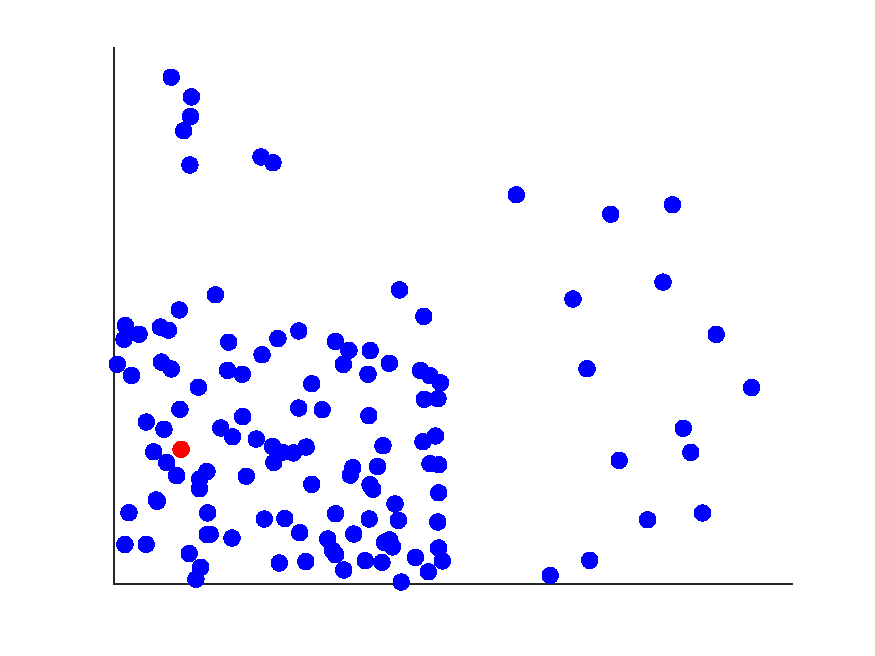
\includegraphics[width=0.45\textwidth]{knn1.pdf}}
		\hfill
		\subfloat[]{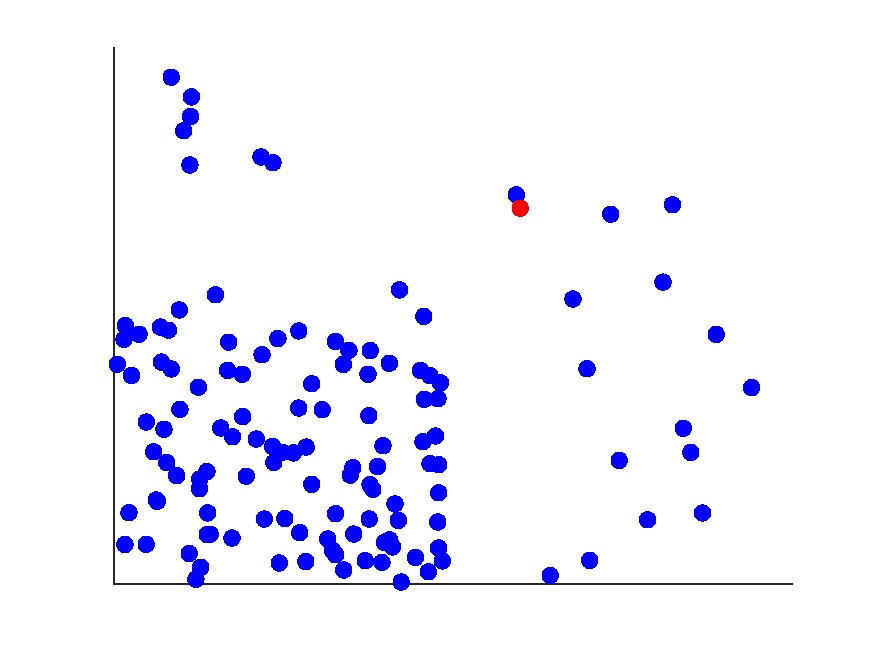
\includegraphics[width=0.45\textwidth]{knn2.pdf}}
		\caption{Motivation for adaptively picking anchor points. In the two scenarios above, the same distribution of anchor points are given (represented by blue dots). The new data point to be estimated is shown as a red dot. Intuitively, in the left scenario it would be resonable to invole more anchor points in the local coding phase while in the right scenario considering fewer anchor points may relieve unreliable estimation of the membership of distint anchor points.}
	\end{figure}
	 Moreover, the anchor points pick and local coding are seperate phases in former localized soft-assignment coding. To address this issue, we propose a unified local coding schema where the number of anchor points and local coding coordinate for each nearest anchor point are optimized in a joint fashion.
	
	To begin with, we first introduce the optimization problem for the local coding coordinates $\gamma_{\x,\v}$. Recall we seek to find the best local approximation in a sense of minimizing the distance between this approximation and the ground truth. Let $\Theta(\x)$ denotes the classifier varying according to the location of data point $\x$.
	\begin{equation}
	\Theta(\x) = \w(\x) + b(\x).
	\end{equation}
	Assume that for any data point $\x$, the ground truth holds that $\Theta_{\x}^* = \Theta(\x) + \epsilon_{\x}$, where $\Theta(\cdot)$ is a Lipschitz continuous function that for any $\x_1, \x_2 \in \mathbb{R}^p$:
	\begin{equation}
	\abs{\Theta(\x_1)-\Theta(\x_2)} \leq L \cdot d(\x_1,\x_2).
	\end{equation}
	where $d(\cdot,\cdot)$ is distance function, so long as defined on any valid metric space. $\epsilon_i$ denotes noise terms and it holds that $\mathbb{E}[\epsilon_{\x}|\x]=0$ and $\abs{\epsilon_{\x}} \leq b$ from some given $b > 0$. Specifically, to minimize the absolute distance between our local linear classifier approximation and the ground truth, we obtain the following optimization problem:
	\begin{equation}
	\min_{\gamma_{\x,\v}} \abs*{\sum_{i=1}^m\gamma_{\x,\v_i}\Theta_{\v_i}^*- \Theta(\x)} \quad s.t. \sum_{i=1}^m\gamma_{\x,\v_i}=1 \quad \mbox{and} \quad \gamma_{\x,\v_i} \geq 0, \forall i.
	\end{equation} 
	Decomposing the above objective into a sum of bias and variance terms, we can transform it into
	\begin{equation}
	\begin{split}
	&\abs*{\sum_{i=1}^m\gamma_{\x,\v_i}\Theta_{\v_i}^*- \Theta(\x)} \\ {}=&\abs*{\sum_{i=1}^{m}\gamma_{\x,\v_i}(\Theta_{\v_i}^*-\Theta(\v_i)+\Theta(\v_i))-\Theta(\x)} \\
	{}=&\abs*{\sum_{i=1}^m\gamma_{\x,\v_i}\epsilon_{\v_i} + \sum_{i=1}^m\gamma_{\x,\v_i}(\Theta(\v_i)-\Theta(\x))}\\
	\leq{}& \abs*{\sum_{i=1}^m\gamma_{\x,\v_i}\epsilon_{\v_i}} + \abs*{\sum_{i=1}^m\gamma_{\x,\v_i}(\Theta(\v_i)-\Theta(\x))}\\
	\leq{}& \abs*{\sum_{i=1}^m\gamma_{\x,\v_i}\epsilon_{\v_i}} +
	L\sum_{i=1}^{m}\gamma_{\x,\v_i} d(\v_i,\x).
	\end{split}
	\end{equation}
	By Hoeffding inequality if follows that $\abs*{\sum_{i=1}^m\gamma_{\x,\v_i}\epsilon_{\v_i}} \leq C\norm{\boldsymbol{\gamma}_{\x,\v}}$ for $C=b\sqrt{2\log{\frac{2}{\delta}}}$, w.p. at least $1-\delta$. With a guarantee for solving the original objective with a high probability, we can obtain the new optimization problem:
	\begin{equation}
	\min_{\boldsymbol{\gamma}_{\x,\v}} C(\norm{\boldsymbol{\gamma}_{\x,\v}} + \boldsymbol{\gamma}_{\x,\v}^T \boldsymbol{\eta}) \quad s.t. \sum_{i=1}^m\gamma_{\x,\v_i}=1 \quad \mbox{and} \quad \gamma_{\x,\v_i} \geq 0, \forall i.
	\end{equation}
	Where $\boldsymbol{\eta}=\{Ld(\x,\v_1)/C,...,Ld(\x,\v_m)/C\}$. Considering the above objective's Lagrangian:
	\begin{equation*}
	L(\boldsymbol{\gamma}_{\x,\v},\boldsymbol{\theta},\lambda) = \norm{\boldsymbol{\gamma}_{\x,\v}} + \boldsymbol{\gamma}_{\x,\v}^T \boldsymbol{\eta} + \lambda(1-\sum_{i=1}^m\boldsymbol{\gamma}_{\x,\v_i}) - \sum_{i=1}^m\theta_i\gamma_{\x,\v_i}.
	\end{equation*}
	where $\lambda \in \mathbb{R}$ and $\theta_1,...,\theta_m \geq 0$ are the Lagrange multipliers. Since the optimization problem is convex. We can employ KKT conditions to find its global minimum. Take the derivation of $L(\boldsymbol{\gamma}_{\x,\v},\theta,\lambda)$ with respect to $\gamma_{\x,\v}$, we can get: 
	\begin{equation}
	\frac{{\gamma}_{\x,\v_i}^*}{\norm{\boldsymbol{\gamma}_{\x,\v}^*}} = \lambda - \eta_i + \theta_i.
	\end{equation}
	Let $\boldsymbol{\gamma}_{\x,\v}^*$ be the optimal local coding coordinates. According to the KKT conditions, if $\gamma_{\x,\v_i}^* \ge 0$ then $\theta_i=0$. Otherwise, for any $i$ such that $\gamma_{\x,\v_i}^* = 0$ it follows that $\theta_i \geq 0$, which implies $\lambda \leq \eta_i$. Combine the constraint $\sum_{i=1}^m\gamma_{\x,\v_i}=1$ with Equation (18) we can obtain:
	\begin{equation}
	\gamma_{\x,\v_i}^* = \frac{\lambda-\eta_i}{\sum_{\gamma_{\x,\v_i}^*>0}(\lambda-\eta_i)}.
	\end{equation}
	It demonstrates that the optimal weight $\gamma_{\x,\v_i}^*$ of anchor point $\v_i$ is proportional to $-d(\x,\v_i)$. It is consistent with intuition and previous soft-assignment coding schema, like the Gaussian-shaped coding schema used in \cite{4}, which has a different weight decay though. Moreover, in our coding schema, the ``early-cut-off'' strategy is adptive according to each data point $\x$. Specifically, only nearest anchor points the satisfies $\lambda-\eta_i>0$ contributes to encoding while other distant anchor points' weights are all set to zero, which is quite different from the conventional localized soft-assignment coding where the number of anchor points involved in encoding is predefined and fixed for the whole dataset.
	
	The solution to finding the optimal distance threshold $\lambda$ is simple. By squaring and summing Equation (18) over all the nonzero entries of $\gamma_{\x,\v}^*$, we get
	\begin{equation}
	1= \sum_{\gamma_{\x,\v_i}^*>0}\frac{(\gamma_{\x,\v_i}^*)^2}{\norm{\boldsymbol{\gamma}_{\x,\v}^*}^2}=\sum_{\gamma_{\x,\v_i}^*>0}(\lambda-\eta_i)^2.
	\end{equation}
	which is equivalent to $k^*\lambda^2-2\lambda\sum_{i=1}^{k^*}\eta_i+(\sum_{i=1}^{k^*}\eta_i^2-1)=0$. Solve this equation with respect to $\lambda$ we get
	\begin{equation}
	\lambda=\frac{1}{k^*}\Bigg(\sum_{i=1}^{k^*}\eta_i+\sqrt{k^*+\bigg(\sum_{i=1}^{k^*}\eta_i\bigg)^2-k^*\sum_{i=1}{k^*}\eta_i^2}\Bigg).
	\end{equation}
	where $k^*$ denotes the number of $k$ smallest nonzero value of $\boldsymbol{\eta}$. Finally, we can give our optimized localized soft-assignment coding algorithm, follows the similar method in \cite{6}, the key idea is to greedily add neighbors according to their distance from $\x$ until the stopping criterion is met.
	\begin{algorithm}[H]
		\caption{Optimized Localized Soft-assignment Coding Algorithm}
		\begin{algorithmic}
			\REQUIRE data point $\x$, anchor point $\V=\{\v_1,...,\v_m\}$
			\ENSURE The number of nearest anchor point $k^*$ and corresponding weight $\boldsymbol{\gamma}_{\x,\v}$
			\STATE Compute the vector of ordered distance $\boldsymbol{\eta} \in \mathbb{R}^m$ and sort $\boldsymbol{\eta}$ by ascending order.
			\STATE Initialize $\lambda_0=\eta_1+1,k=0$
			\WHILE {$\lambda_k>\eta_{i+1}$ and $k\leq n-1$}
			\STATE Update: $k\leftarrow k+1$
			\STATE Compute: $\lambda=\frac{1}{k}\Bigg(\sum_{i=1}^{k}\eta_i+\sqrt{k+\bigg(\sum_{i=1}^{k}\eta_i\bigg)^2-k^*\sum_{i=1}{k}\eta_i^2}\Bigg)$
			\ENDWHILE
			\STATE compute the local coding coordinates $\boldsymbol{\gamma}_{\x,\v}$ based on Equation (19)
		\end{algorithmic}
	\end{algorithm}
	\subsection{The Stochastic Gradient Descent Algorithm for LLC-JO}
	We next integrate the above refined localized soft-assignment coding schema into LLC-SAPL \cite{4}, leading to a optimized framework for adaptively learning the optimal number of anchor points and corresponding weights according to each data point. To solve objective (12), we use Stochastic Gradient Descent (SGD) in that it is simple and efficient. What's more, learning in an online fashion is favorable in large datasets. Specifically, at each SGD iteration, we randomly sample a data point $\x$ and its corresponding targer $y$, then we update the nearby anchor points $\V$ and correponding classfier's parameters $\Theta(\V)$. As in our optimized localized soft-assignment coding schema, data point $\x$ is approximated as a linear combination of its $k$-nearest anchor points, hence only $k$-nearest anchor points need to be optimized in each update. Note the optimum k anchor points for each data point is picked following Algorithm (1). Here we follows the method in \cite{4}, take the anchor points as parameters like classifier and update each part while fixing the other. To start off, we take partial derivate of $\gamma_{\x,\v_i}^T$ with respect to $\v_i$, then we get a $p\times m$ matrix, among which only k columns are nonzero. The $i$th column of $\frac{\partial\gamma_{\x,\v}}{\partial\z_i}$ goes like:
	\begin{equation}
	\frac{\s\mu(\lambda-\mu d(x,\v_i)-\sum_{\gamma_{\x,\v_i}>0}(\lambda-\mu d(x,\v_i)))}{\sum_{\gamma_{\x,\v_j}>0}(\lambda-\mu d(x,\v_j))^2}.
	\end{equation}
	where $\s = \frac{\partial d(\x,\v_i)}{\partial \v_i}$ and $\mu = L/C$, namely the Lipschitz to noise ratio. The other nonzero columns are computed as:
	\begin{equation}
	-\frac{\s\mu}{\sum_{\gamma_{\x,\v_j}>0}(\lambda-Ld(\x,\v_j))^2}.
	\end{equation}
	where $\v_j$ belongs to the $k$-nearest neighbors of $\x$ and it is not equal to $\v_i$. Then we can update anchor points $\v_i$ via the following formula:
	\begin{equation}
	\v_i^{(t+1)} \leftarrow \v_i^{(t)} + \frac{1}{\rho(t+t_0)}y\frac{\partial \gamma_{\x,\v}}{\partial \v_i}(\W^{(t)}\x + \b^{(t)}).
	\end{equation}
	where $t$ denotes the current SGD iteration number and $t_0$ is a positive constant that avoids too large steps in the first few iterations. We follow the optimal learning rate schema $\frac{1}{\rho(t+t_0)}$ given by \cite{13} \cite{14}.
	The classifier variable $W$ and $b$ are updated as:
	\begin{equation}
	\W^{(t+1)} \leftarrow \W^{(t)} + \frac{1}{\rho(t+t_0)}y(\gamma_{\x,\v}\x^T).
	\end{equation}
	\begin{equation}
	\b^{(t+1)} \leftarrow \b^{(t)} + \frac{1}{\rho(t+t_0)}y\gamma_{\x,\v}.
	\end{equation}
	To avoid overfitting ,we take the same regularization method in \cite{13} to update the weight matrix $\W$ every $skip$ iterations by:
	\begin{equation}
	\W^{(t+1)} \leftarrow \W^{(t+1)} - \frac{skip}{t+t_0}\W^{(t+1)}.
	\end{equation} 
	At last, we give the complete algorithm for the locally linear classifier based on the optimized localized soft-assignment coding schema.
	\begin{algorithm}[H]
		\caption{Joint optimized Locally Linear Classifier (LLC-JO)}
		\begin{algorithmic}
			\REQUIRE Training Data ${(\x_n,y_n)}_{n=1}^N \subset \mathbb{R}^p \times \{-1,1\}$, the number of anchor points $m$, parameters $\lambda,t_0,skip$ and Lipschitz to noise ration $\mu$
			\ENSURE Classifier variables $\W, \b$ and anchor points $\v$
			\STATE Initialize anchor points $\v$ by K-means.
			\STATE Set: t=0
			\WHILE {no convergence}
				\STATE Sample a data point $\x$ randomly.
				\STATE Compute the local coordinate $\gamma_{\x,\v}$ according to Algorithm (1).
				\STATE Compute hinge loss $L = 1-y\boldsymbol{\gamma}_{\x,\v}^T(\W\x + \b)$.
				\IF {$L>0$}
					\FOR {each nearest anchor point $\v_i$ to data point $\x$}
						\STATE update $\v_i$ via Equation (24).
						\STATE update the Classifiers' parameters $\W$ and $\b$ via Equation (25) and (26), respectively.
					\ENDFOR
				\ENDIF
				\IF {$t$ mod $skip == 0$}
					\STATE update weight matrices $\W$ via Equation (27).
				\ENDIF
				\STATE Update: $t\leftarrow t+1$
			\ENDWHILE
		\end{algorithmic}
	\end{algorithm}
	The algorithm (2) is easily extended to multi-class classfication task with a little modification to the objective and SGD update equation. We follow the same assumption in \cite{4} that the different weight matrices and bias vectors for different classes can be learnt while sharing the same anchor points among class, which saves signficant computational overhead for multi-class classfication comparing to naive one-vs-all strategy.
	\section{Experiment}
	To evaluate the performance of our LLC-JO Algorithm, we use several benchmarks, including both binary classfication and multi-class classification tasks.
	\subsection{Experimental Setup}
	\subsubsection{Datasets \& Evaluation Metrics.}
	We conduct experiments on five real-world datasets: Banana, Magic04, IJCNN, W8a, USPS, LETTER. Banana dataset can be found at \footnote{http://mldata.org/repository/data/viewslug/banana-ida/} while the rest of datasets are obtained from the LibSVM website \cite{15}.  All the datasets are normalized to have zero mean and unit variance in each dimension. The statistics of the datasets after preprocessing are summarized in Table 1.
	\begin{table}
		\centering
		\begin{tabu} to \textwidth {|X[c]| X[c]| X[c]| X[c]| X[c]|}
			\hline
			Dataset              & \#Training & \#Test & \#feature &\#class\\
			\hline
			Banana 		   	& 3533 & 1767 & 2 & 2  \\
			Magic04     	& 12680 & 6340 & 10 & 2  \\
			IJCNN           	& 49990 & 91701 & 22 & 2  \\
			W8a           	& 49479 & 14951 & 300 & 2  \\
			USPS			& 7291 & 2007 & 256 & 10  \\
			\hline
		\end{tabu}
		\caption{Basic statistics of datasets}
	\end{table}
	To make a fair comparison, all the algorithms are repeated over 5 experimental runs of different random permutation. For performance metric, we evaluate the performance of each method for classfication task by measuring hinge loss on test dataset, defined as:
	\begin{equation*}
	hingeloss_{test} = \frac{1}{N}\sum_{i=1}^N\max(0,1-y_ip_i).
	\end{equation*}
	where $N$ is the number of samples in test dataset, $y_i$ indicates the label while $p_i$ denotes the classifier's predication.
	\subsubsection{Model Comparsion.}
	In our experiments, we compare the following methods:
	\begin{itemize}
		\item \textbf{SVM}: Standard linear SVM without any local coding embedding, which is baseline method for locally linear classifer based on local coding schema.
		\item \textbf{LLSVM}: Locally Linear SVM without any decoupled optimization method \cite{2}. We first initialize the anchor points by K-means clustering and fixed for the following learning procedure. Then we encode the training data with local soft-assignment coding and optimize the classifiers' parameters. This method is a baseline to validate the efficacy of \textbf{LLC-SAPL}.
		\item \textbf{LLC-SAPL}: Locally Linear Classifier with Supervised Anchor Points Learning \cite{4}. This method optimize anchor points just like the classifiers' parameters but using a fixed localized soft-assignment coding schema, which indicates the number of anchor points is fixed for the whole dataset. This algorithm can be viewed as a strong baseline for the locally-linear-classifier-related algorithm.
		\item \textbf{LLC-JO}: The proposed Locally linear Classifier based on a optimized localized soft-assignment coding schema in Algorithm (2).
	\end{itemize}
	\subsubsection{Hyper-parameter Settings.}
	For parameter settings, we perform grid search to select the best parameters for each algorithm on the training set. To be specific, the hyper-parameters including: learning rate related parameters in SGD-QN $\rho \in \{10^{-5},10^{-4}, 10^{-3}, 10^{-2},10^{-1}\}, t_0 \in \{10^2,10^3,10^4,10^5\}$, regularization related parameter $skip \in \{10^1,10^2,10^3,10^4\}$, the nearest number of anchor points to be updated in \textbf{LLSVM} and \textbf{LLC-SAPL} $k \in \{1,3,5,10,20\}$, Lipschitz to noise ratio $\mu \in \{0.1,0.2,0.4,0.6,0.8,1,5,10,100\}$. To be fair, we adopt squared Euclidean distance as distance function in local soft-assignment coding and our proposed optimizd coding schema. We adopt the same number of anchor points $m \in \{50,100,200\}$ in the above methods. Cumulative hinge loss is used to demonstrate the learning process for all the methods.
	\subsection{Experimental Results \& Analysis}
	The comparison results in terms of training hinge loss, test hinge loss and accuracy for each benchmark are presented in Table 2-5.
	It is clear that LLC-JO method based on optimized local soft-assignment coding schema achieves better performance comparing to the three other baselines. LLSVM beats linear SVM proves the efficacy of local coding embedding, while LLC-SAPL refines LLSVM by adding supervised anchor point learning instead of learning in a decoupled way. LLC-JO not only integrates supervised anchor point learning, but also employ a joint optimized locing coding schema, where the optimum number of anchor points and corresponding local coordinates are learning adaptively.
	
	
	\begin{table}
		\begin{tabu} to \textwidth {|X[c]| X[c]| X[c]| X[c]|}
			\hline
			Banana              & Train loss & Test loss & Acc(\%) \\
			\hline
			\textbf{SVM} 		   	&0.9061$\pm$0.0000  &0.8958$\pm$0.0018  & 55.40 $\pm$ 0.00   \\ \hline
			\textbf{LLSVM}     		&0.3139$\pm$0.0027  &0.2547$\pm$0.0042  & 89.16 $\pm$ 0.13   \\ \hline
			\textbf{LLC-SAPL}       &0.2930$\pm$0.0019  &0.2307$\pm$0.0050  & \textbf{90.03 $\pm$ 0.31}  \\ \hline
			\textbf{LLC-JO}         &\textbf{0.2416$\pm$0.0016}  &\textbf{0.2103$\pm$0.0034}  & \textbf{90.03 $\pm$ 0.34}  \\ \hline
		\end{tabu}
		\caption{Experimental results on Banana dataset}
	\end{table}

	\begin{table}
		\begin{tabu} to \textwidth {|X[c]| X[c]| X[c]| X[c]|}
			\hline
			Magic04              & Train loss & Test loss & Acc(\%) \\
			\hline
			\textbf{SVM} 		   	&0.4874$\pm$0.0005  &0.5022$\pm$0.0020  &78.35 $\pm$ 0.46   \\ \hline
			\textbf{LLSVM}     		&0.4105$\pm$0.0019  &0.4017$\pm$0.0102  &82.97 $\pm$ 0.42   \\ \hline
			\textbf{LLC-SAPL}       &0.3604$\pm$0.0019  &0.3720$\pm$0.0057  &83.18 $\pm$ 0.29   \\ \hline
			\textbf{LLC-JO}         &\textbf{0.3390$\pm$0.0017}  &\textbf{0.3422$\pm$0.0038}  &\textbf{83.53 $\pm$ 0.28}   \\ \hline
		\end{tabu}
		\caption{Experimental results on Magic04 dataset}
	\end{table}

	\begin{table}
		\begin{tabu} to \textwidth {|X[c]| X[c]| X[c]| X[c]|}
			\hline
			IJCNN              & Train loss & Test loss & Acc(\%) \\
			\hline
			\textbf{SVM} 		   	&0.1930$\pm$0.0000  &0.1896$\pm$0.0000  & 90.50 $\pm$ 0.00  \\ \hline
			\textbf{LLSVM}     		&0.1072$\pm$0.0014  &0.0947$\pm$0.0009  & 96.18 $\pm$ 0.25  \\ \hline
			\textbf{LLC-SAPL}       &0.0970$\pm$0.0027  &0.0858$\pm$0.0200  & 96.97 $\pm$ 0.68  \\ \hline
			\textbf{LLC-JO}         &\textbf{0.0942$\pm$0.0007}  &\textbf{0.0716$\pm$0.0074}  & \textbf{97.12 $\pm$ 0.51}   \\ \hline
		\end{tabu}
		\caption{Experimental results on IJCNN dataset}
	\end{table}

	\begin{table}
		\begin{tabu} to \textwidth {|X[c]| X[c]| X[c]| X[c]|}
			\hline
			W8a              & Train loss & Test loss & Acc(\%) \\
			\hline
			\textbf{SVM} 		   	&0.0409$\pm$0.0001  &0.0415$\pm$0.0000  &98.15 $\pm$ 0.02   \\ \hline
			\textbf{LLSVM}     		&0.0319$\pm$0.0002  &0.0275$\pm$0.0004  &98.82 $\pm$ 0.04   \\ \hline
			\textbf{LLC-SAPL}       &0.0268$\pm$0.0002  &0.0201$\pm$0.0003  &99.03 $\pm$ 0.03   \\ \hline
			\textbf{LLC-JO}         &\textbf{0.0258$\pm$0.0007}  &\textbf{0.0194$\pm$0.0008}  &\textbf{99.08 $\pm$ 0.02}   \\ \hline
		\end{tabu}
		\caption{Experimental results on W8a dataset}
	\end{table}

	To further illustrate the convergence of different algorithms, we give the online cumulative hinge loss performance of different methods in Figure 2. From the results, we can see that LLC-JO outperforms the other algorithms. From those online training curves, we can validate the optimized localized soft-assignment achieve a tight coupling of the classifier and local coding technique.
	
	\begin{figure}[!tbp]
		\centering
		\subfloat[Magic04]{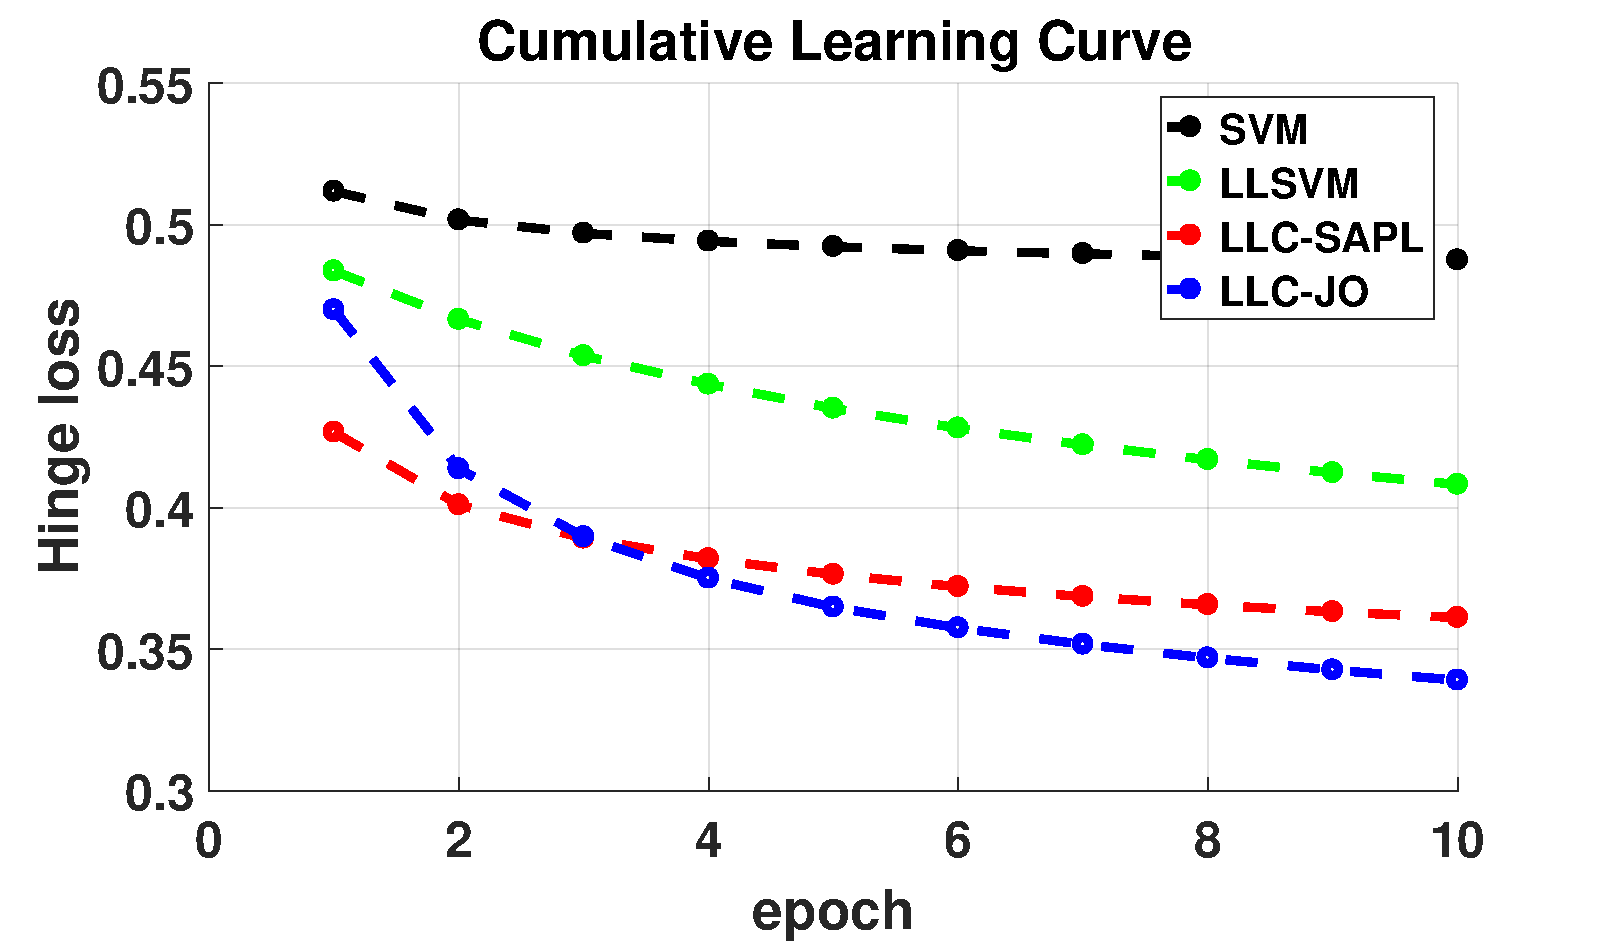
\includegraphics[width=0.5\textwidth]{magic04.pdf}}
		\hfill
		\subfloat[IJCNN]{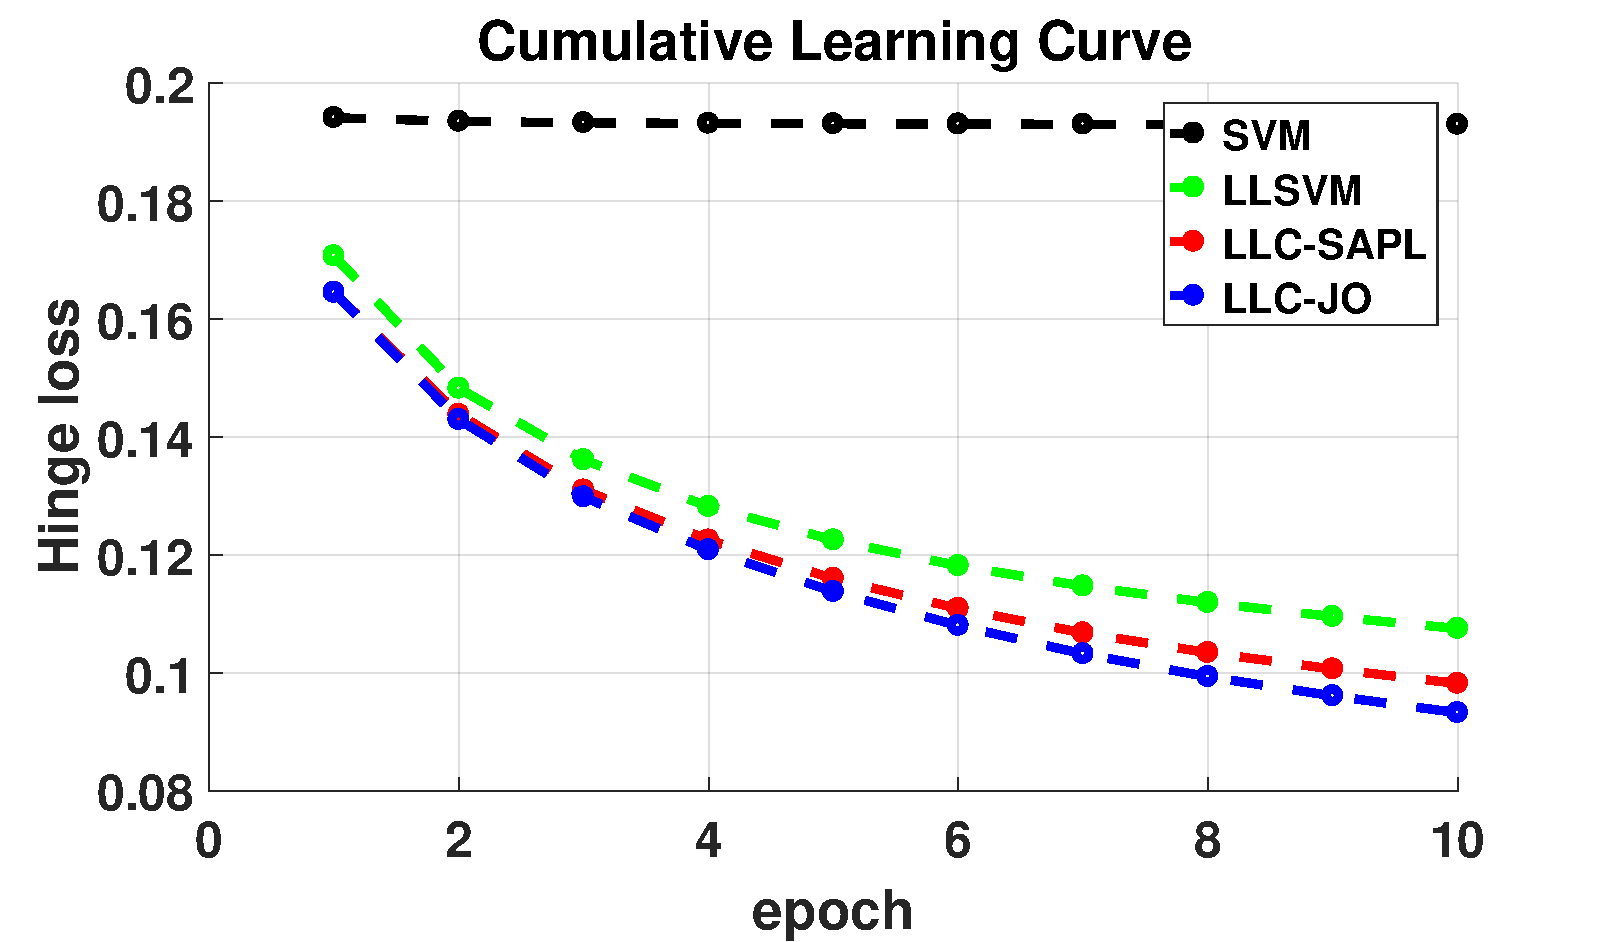
\includegraphics[width=0.5\textwidth]{ijcnn.pdf}}
		\caption{Cumulative Hinge Loss in learning process on Magic04 and IJCNN dataset.}
	\end{figure}

	To illustrate the combination of supervised anchor point learning and optimum local coding coordinates learning, we give the average number of nearest neighbors learning curve in Figure 3. As the figure shows, the average number of anchor points involved in coding phase is decreasing and prone to convergence. The reason may be that during the learning process, the anchor points are being optimized and gain more discriminative information of the whole dataset. These two methods contribute to a more stable and efficient online learning algorithm for locally linear classfiers.
	\begin{figure}[!tbp]
		\centering
		\subfloat[Magic04]{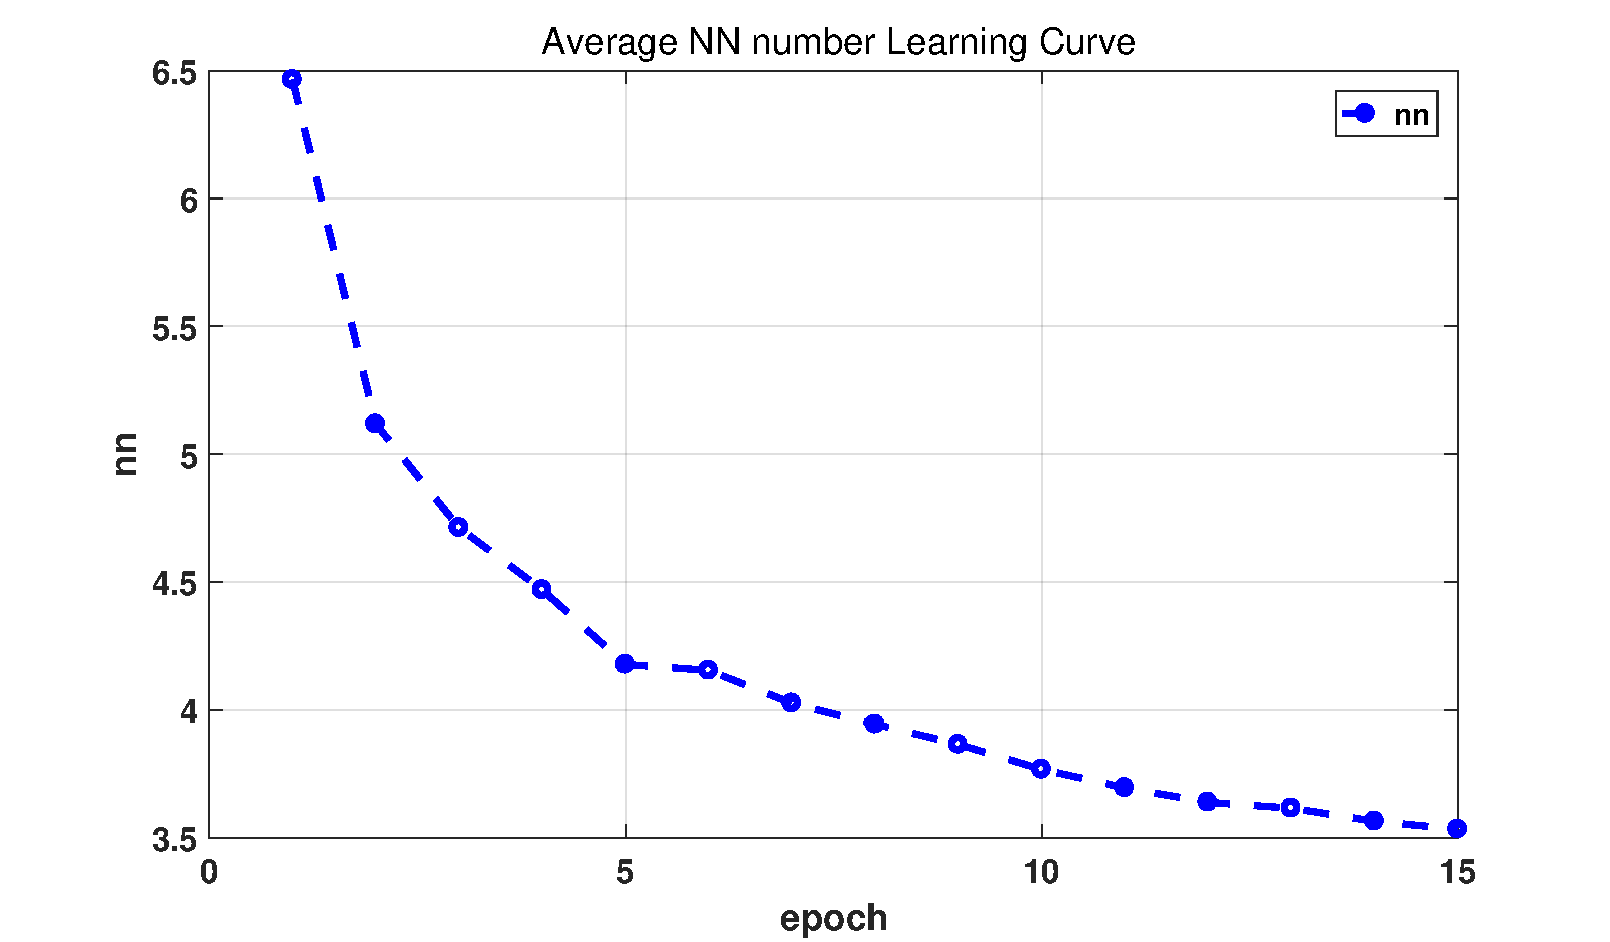
\includegraphics[width=0.5\textwidth]{magic04_nn.pdf}}
		\hfill
		\subfloat[IJCNN]{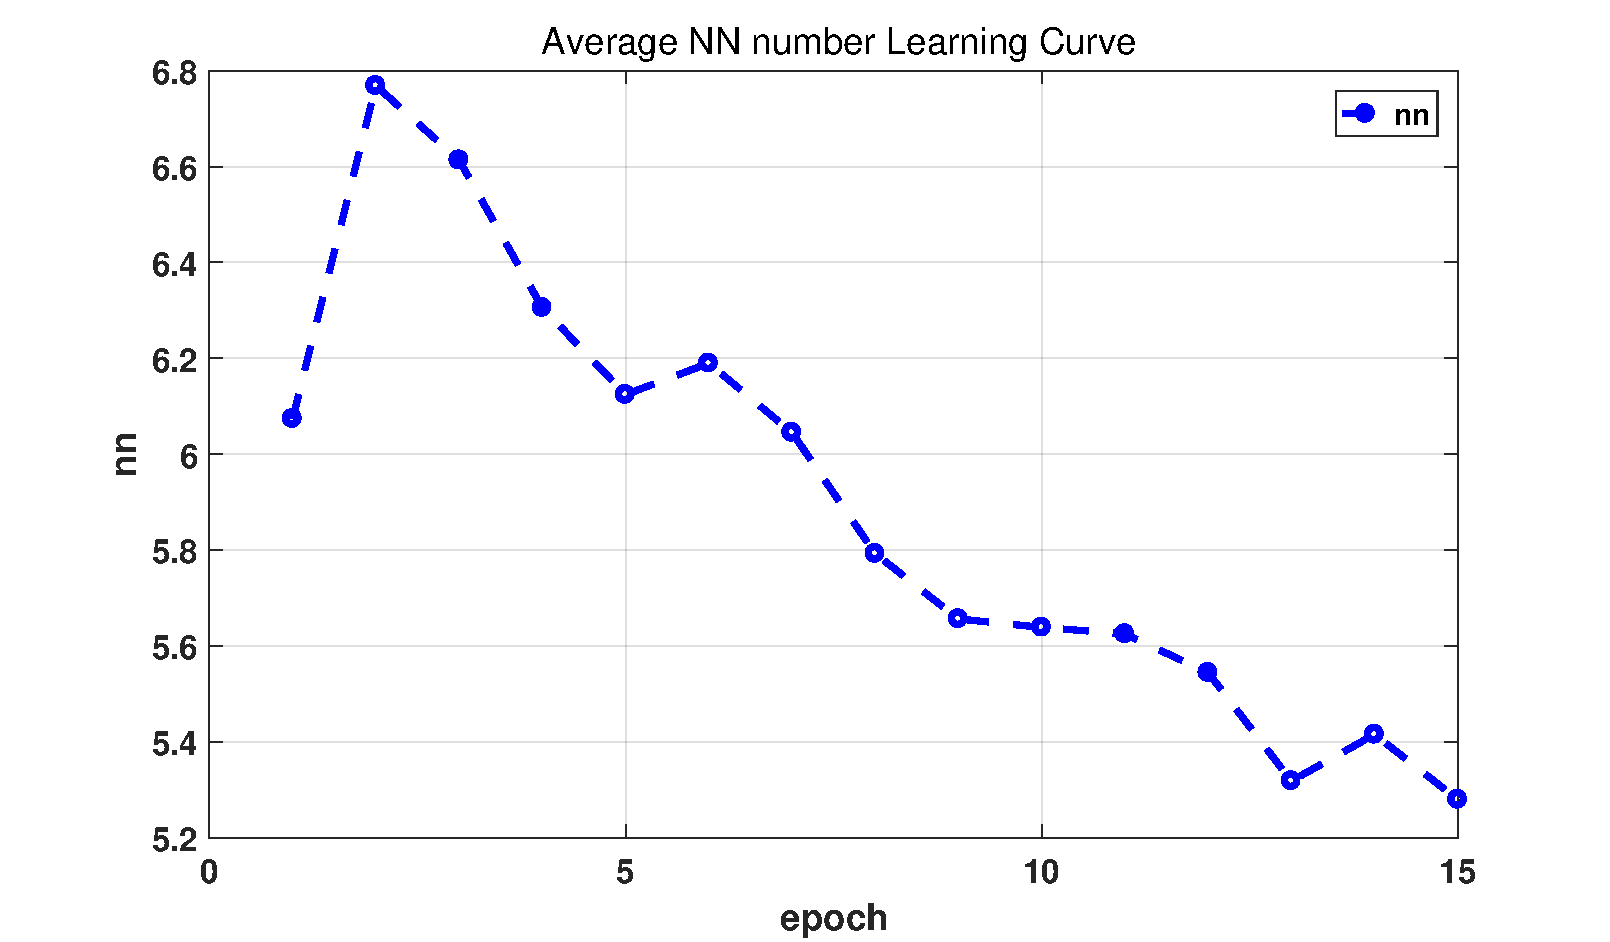
\includegraphics[width=0.5\textwidth]{ijcnn_nn.pdf}}
		\caption{Cumulative Average Number of Nearest Neighbors in learning process on Magic04 and IJCNN dataset.}
	\end{figure}

	\section{Conclusion}
	In this paper, we propose an optimized local soft-assignment coding schema. Different existing localized soft-assignment coding, we formulate a joint optimization over anchor points, local coding coordinates and classifiers' variables by minimizing the distance of local approximation to the ground truth. In this novel coding schema, the anchor points and corresponding local coding coordinates are optimized for each data point adaptively. This design gives full consideration to that the local manifolds may vary from data point to data point.  Based on the new coding schema, we give the algorithm for joint optimized locally linear classifier(LLC-JO). Experiment results on several benchmarks demonstrates that our algorithm achieves lower hinge loss and better predicitive accuracy than other competitive methods which employ a fixed local coding schema.
	\begin{thebibliography}{1}
		\bibitem{1}
		Schölkopf B, Smola A J. Learning with kernels: support vector machines, regularization, optimization, and beyond[M]. MIT press, 2002.
		\bibitem{2}
		Ladicky L, Torr P. Locally linear support vector machines[C]//Proceedings of the 28th International Conference on Machine Learning (ICML-11). 2011: 985-992.
		\bibitem{3}
		Yu K, Zhang T, Gong Y. Nonlinear learning using local coordinate coding[C]//Advances in neural information processing systems. 2009: 2223-2231.
		\bibitem{4}
		Mao X, Fu Z, Wu O, et al. Optimizing Locally Linear Classifiers with Supervised Anchor Point Learning[C]//IJCAI. 2015: 3699-3706.
		\bibitem{5}
		Zhou X, Cui N, Li Z, et al. Hierarchical gaussianization for image classification[C]//Computer Vision, 2009 IEEE 12th International Conference on. IEEE, 2009: 1971-1977.
		\bibitem{6}
		Anava O, Levy K. k*-Nearest Neighbors: From Global to Local[C]//Advances in Neural Information Processing Systems. 2016: 4916-4924.
		\bibitem{7}
		Cover T, Hart P. Nearest neighbor pattern classification[J]. IEEE transactions on information theory, 1967, 13(1): 21-27.
		\bibitem{8}
		Liu L, Wang L, Liu X. In defense of soft-assignment coding[C]//Computer Vision (ICCV), 2011 IEEE International Conference on. IEEE, 2011: 2486-2493.
		\bibitem{9}
		Van Gemert J, Geusebroek J M, Veenman C, et al. Kernel codebooks for scene categorization[J]. Computer Vision–ECCV 2008, 2008: 696-709.
		\bibitem{10}
		Van Gemert J C, Veenman C J, Smeulders A W M, et al. Visual word ambiguity[J]. IEEE transactions on pattern analysis and machine intelligence, 2010, 32(7): 1271-1283.
		\bibitem{11}
		Wang J, Yang J, Yu K, et al. Locality-constrained linear coding for image classification[C]//Computer Vision and Pattern Recognition (CVPR), 2010 IEEE Conference on. IEEE, 2010: 3360-3367.
		\bibitem{12}
		Yu K, Zhang T, Gong Y. Nonlinear learning using local coordinate coding[C]//Advances in neural information processing systems. 2009: 2223-2231.
		\bibitem{13}
		Bordes A, Bottou L, Gallinari P. Sgd-qn: Careful quasi-newton stochastic gradient descent[J]. Journal of Machine Learning Research, 2009, 10(Jul): 1737-1754.
		\bibitem{14}
		Shalev-Shwartz S, Singer Y, Srebro N. Pegasos: Primal estimated sub-gradient solver for svm[C]//Proceedings of the 24th international conference on Machine learning. ACM, 2007: 807-814.
		\bibitem{15}
		Chang C C, Lin C J. LIBSVM: a library for support vector machines[J]. ACM Transactions on Intelligent Systems and Technology (TIST), 2011, 2(3): 27.
	\end{thebibliography}
\end{document}